\section{Natural Language Processing}
Human language is a symbolic system aimed at the transmission of meaning.
The symbols of a language can be encoded in various ways: sounds gestures writing. \\
\vspace{1em}
NLP is concerned with creating an algorithm that can understand natural language (knowledge acquisition) and communicate with humans.
This can help in various contexts such as translating text,answering questions and creating summaries.
However, understanding natural language is complicated given its ambiguous nature.

\subsection{NLP Levels}
There are several levels of NLP.
The format must be made understandable to the algorithm.
\begin{center}
    \begin{tabular}{c}
        \\ 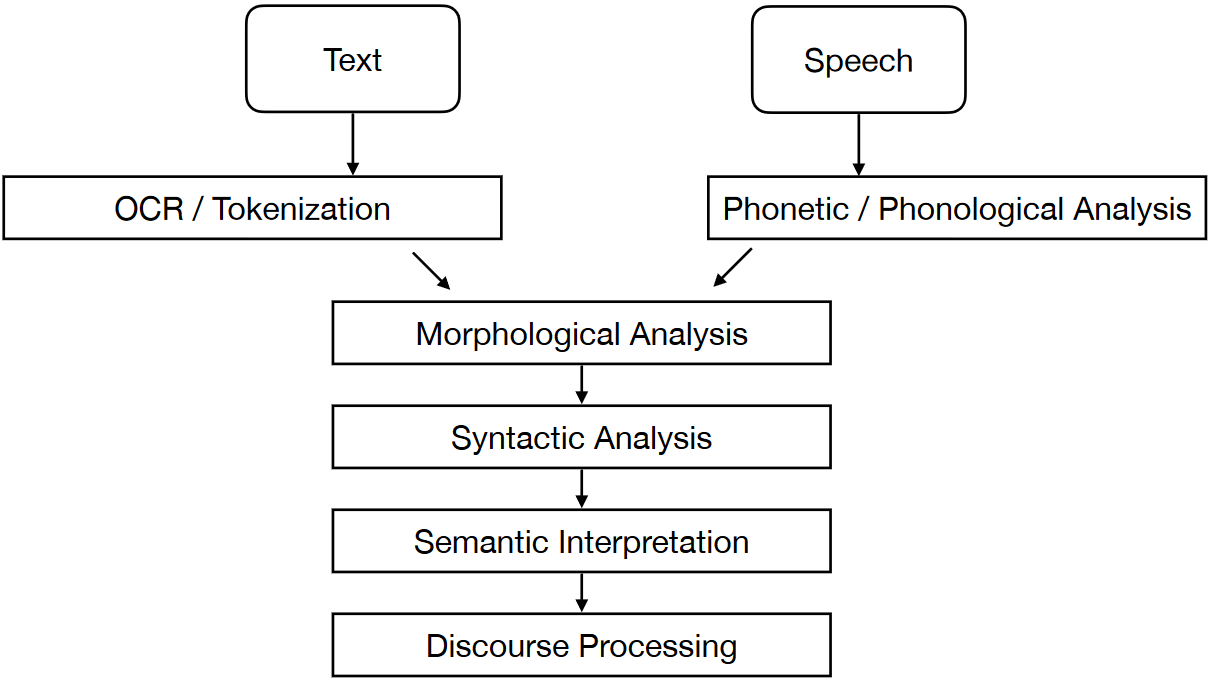
\includegraphics[width=0.9\textwidth]{images/NPL1.png} \\ \\
    \end{tabular}
\end{center}

\subsection{NLP Applications}
\begin{itemize}
    \item Spell checking, keyword search, finding synonyms
    \item Extracting information from documents or websites
    \item Text classification, reading level of school texts, sentiment analysis of longer documents
    \item Machine translation
    \item Conversational agents (spoken dialog)
    \item Question answering
\end{itemize}

\subsection{NLP Fundamental Tasks}
\begin{itemize}
    \item \textbf{Named entity recognition:} extrapolation and classification of particular words taken from a text within specific groups.
    \item \textbf{Entity mention detection:} classification of multiple entities into different groups.
    \item \textbf{Relation extraction:} association between different classes of vocabulary.
    \item \textbf{Coreference resolution:} association of a particular entity with a reference to it.
\end{itemize}

\subsection{Knowledge Acquisition}
NLP in terms of information seeking tasks:
\begin{itemize}
    \item Text classification
    \item Information retrieval
    \item Information extraction
\end{itemize}
A common factor in addressing these tasks is the use of language models, models that predict the probability distribution of language expressions.

\newpage